\section{Discussion \& Threats to Validity}

\subsection{Runtime Throughput}

A limitation of the current workflow is that test generation, minimization,
and sorting can reduce overall throughput.
Each generated subject may require many browser executions, especially during
minimization, where the current approach removes elements and declarations one
at a time.
This process is effective, but it can be expensive when a subject contains
many HTML nodes or CSS declarations.

A more efficient approach could use divide-and-conquer minimization.
Instead of testing each element individually, the minimizer could first try
removing larger groups of HTML nodes or CSS declarations.
If removing a group fails to preserve the bug, the algorithm could then test
smaller groups within that region.
This strategy could reduce the number of browser executions needed to produce
a compact test case.

Throughput could also be improved by parallelizing generation, minimization,
and sorting.
For example, candidate bugs could be placed into a queue for minimization
while other workers continue generating and testing new subjects.
However, this introduces additional challenges, including resource
management, synchronization, and avoiding duplicate reports.

This limitation affects the number of tests the tool can execute in a fixed
amount of time.
However, it does not invalidate the results, since the current workflow still
generates, detects, minimizes, and organizes reproducible browser-layout bugs.

\subsection{Browser Coverage}

Another threat to validity is that the results depend on which browsers are
supported and tested.
Supporting a browser requires browser-specific configuration, a compatible
automation driver, and reliable access to layout information used by the
oracle.
These requirements make it practical to test major browsers with good
WebDriver support, but they make it harder to test uncommon browsers, older
versions, or browsers with incomplete automation support.

This means that the tool may miss bugs that only appear in less common browser
engines or older browser versions.
These browsers may contain defects that are not found in Chromium,
WebKit/Safari, or Firefox, especially if they receive less testing and
maintenance.
As a result, the findings should not be interpreted as covering all possible
browser implementations.

At the same time, focusing on major browser engines still provides strong
practical coverage.
The supported Chromium, WebKit/Safari, and Firefox configurations cover most
browser usage.
Worldwide in May 2026, Chrome accounted for 70.25\% of browser usage, Safari
for 15.72\%, and Firefox for 5.14\%.
Together, these browsers accounted for 91.11\% of
usage~\cite{statcounterBrowserShare2026}.
This leaves 8.89\% of usage outside the main target of \toolname.

\begin{figure}[t]
    \centering
    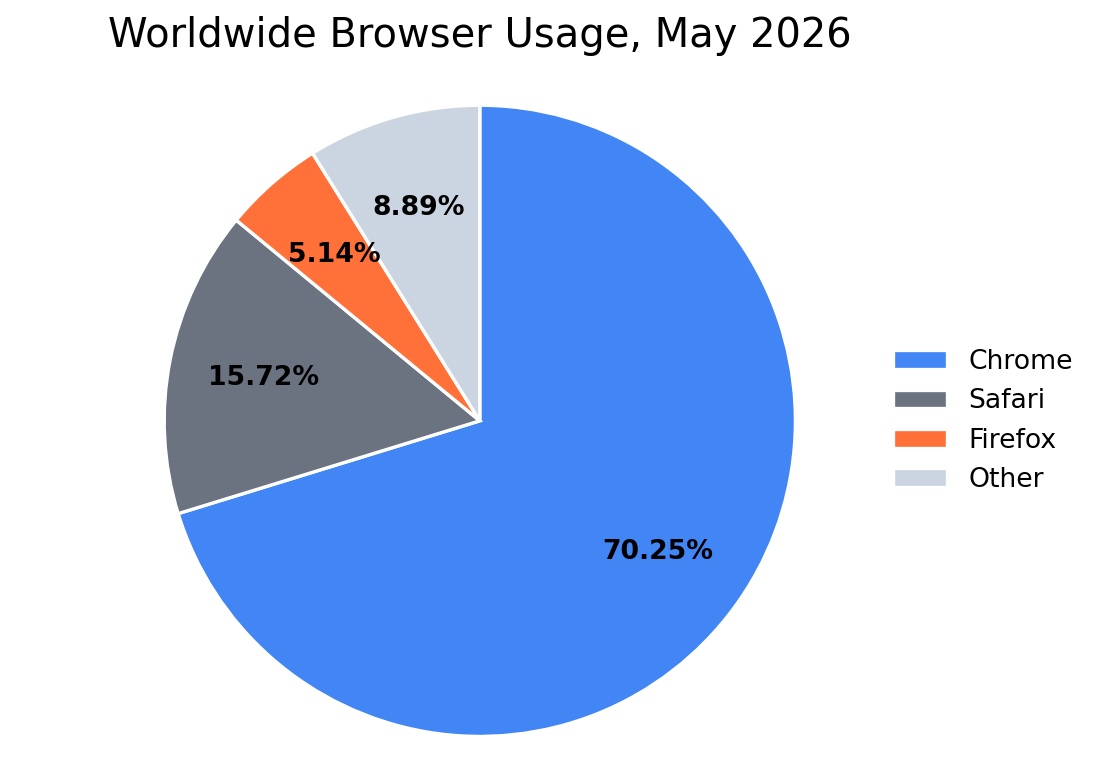
\includegraphics[width=\columnwidth]{figures/worldwide_browser_usage_may_2026.png}
    \caption{Worldwide browser usage in May
    2026~\cite{statcounterBrowserShare2026}.}
    \label{fig:browser-usage-share}
\end{figure}

Therefore, browser coverage is a limitation of the evaluation, but the
current implementation remains useful because it targets the engines with the
largest user populations and the most reliable automation tooling.

\subsection{Novel Bug Discovery Rate}

The bug detection rate directly affects the efficiency of the tool, since a
higher rate produces more candidate bugs per executed test case.
However, repeatedly finding the same underlying defect is less useful than
discovering distinct bugs.
One approach to increasing the bug rate is to identify a stronger static
style-weight configuration before a testing run begins.
Results from earlier runs can identify HTML structures, CSS properties, and
style updates that have produced layout inconsistencies most often.
These observations can then be used to assign greater initial weights to
promising properties while preserving lower probabilities for less
frequently selected properties.
Separately, a feedback-driven system could dynamically adjust style-selection
probabilities while a testing run is running.
It could increase the weights of properties associated with novel layout
discrepancies and reduce the weights of configurations that repeatedly
produce uninteresting or duplicate results.
The system should retain a degree of random exploration so that it does not
become overly focused on known bug patterns.
Despite this, the current random generation strategy remains useful because
it can discover unexpected bug classes without requiring prior knowledge of
effective configurations.
